\documentclass[11pt,]{article}
\usepackage[left=1in,top=1in,right=1in,bottom=1in]{geometry}
\newcommand*{\authorfont}{\fontfamily{phv}\selectfont}
  \usepackage[]{mathpazo}
  
  
  \usepackage[T1]{fontenc}
\usepackage[utf8]{inputenc}



\usepackage{abstract}
\renewcommand{\abstractname}{}    % clear the title
\renewcommand{\absnamepos}{empty} % originally center

\renewenvironment{abstract}
{{%
  \setlength{\leftmargin}{0mm}
  \setlength{\rightmargin}{\leftmargin}%
}%
  \relax}
{\endlist}

\makeatletter
\def\@maketitle{%
  \newpage
  %  \null
  %  \vskip 2em%
    %  \begin{center}%
    \let \footnote \thanks
  {\fontsize{18}{20}\selectfont\raggedright  \setlength{\parindent}{0pt} \@title \par}%
}
%\fi
\makeatother


  
  
  \setcounter{secnumdepth}{0}

      \usepackage{color}
  \usepackage{fancyvrb}
  \newcommand{\VerbBar}{|}
  \newcommand{\VERB}{\Verb[commandchars=\\\{\}]}
  \DefineVerbatimEnvironment{Highlighting}{Verbatim}{commandchars=\\\{\}}
  % Add ',fontsize=\small' for more characters per line
  \usepackage{framed}
  \definecolor{shadecolor}{RGB}{248,248,248}
  \newenvironment{Shaded}{\begin{snugshade}}{\end{snugshade}}
  \newcommand{\AlertTok}[1]{\textcolor[rgb]{0.94,0.16,0.16}{#1}}
  \newcommand{\AnnotationTok}[1]{\textcolor[rgb]{0.56,0.35,0.01}{\textbf{\textit{#1}}}}
  \newcommand{\AttributeTok}[1]{\textcolor[rgb]{0.77,0.63,0.00}{#1}}
  \newcommand{\BaseNTok}[1]{\textcolor[rgb]{0.00,0.00,0.81}{#1}}
  \newcommand{\BuiltInTok}[1]{#1}
  \newcommand{\CharTok}[1]{\textcolor[rgb]{0.31,0.60,0.02}{#1}}
  \newcommand{\CommentTok}[1]{\textcolor[rgb]{0.56,0.35,0.01}{\textit{#1}}}
  \newcommand{\CommentVarTok}[1]{\textcolor[rgb]{0.56,0.35,0.01}{\textbf{\textit{#1}}}}
  \newcommand{\ConstantTok}[1]{\textcolor[rgb]{0.00,0.00,0.00}{#1}}
  \newcommand{\ControlFlowTok}[1]{\textcolor[rgb]{0.13,0.29,0.53}{\textbf{#1}}}
  \newcommand{\DataTypeTok}[1]{\textcolor[rgb]{0.13,0.29,0.53}{#1}}
  \newcommand{\DecValTok}[1]{\textcolor[rgb]{0.00,0.00,0.81}{#1}}
  \newcommand{\DocumentationTok}[1]{\textcolor[rgb]{0.56,0.35,0.01}{\textbf{\textit{#1}}}}
  \newcommand{\ErrorTok}[1]{\textcolor[rgb]{0.64,0.00,0.00}{\textbf{#1}}}
  \newcommand{\ExtensionTok}[1]{#1}
  \newcommand{\FloatTok}[1]{\textcolor[rgb]{0.00,0.00,0.81}{#1}}
  \newcommand{\FunctionTok}[1]{\textcolor[rgb]{0.00,0.00,0.00}{#1}}
  \newcommand{\ImportTok}[1]{#1}
  \newcommand{\InformationTok}[1]{\textcolor[rgb]{0.56,0.35,0.01}{\textbf{\textit{#1}}}}
  \newcommand{\KeywordTok}[1]{\textcolor[rgb]{0.13,0.29,0.53}{\textbf{#1}}}
  \newcommand{\NormalTok}[1]{#1}
  \newcommand{\OperatorTok}[1]{\textcolor[rgb]{0.81,0.36,0.00}{\textbf{#1}}}
  \newcommand{\OtherTok}[1]{\textcolor[rgb]{0.56,0.35,0.01}{#1}}
  \newcommand{\PreprocessorTok}[1]{\textcolor[rgb]{0.56,0.35,0.01}{\textit{#1}}}
  \newcommand{\RegionMarkerTok}[1]{#1}
  \newcommand{\SpecialCharTok}[1]{\textcolor[rgb]{0.00,0.00,0.00}{#1}}
  \newcommand{\SpecialStringTok}[1]{\textcolor[rgb]{0.31,0.60,0.02}{#1}}
  \newcommand{\StringTok}[1]{\textcolor[rgb]{0.31,0.60,0.02}{#1}}
  \newcommand{\VariableTok}[1]{\textcolor[rgb]{0.00,0.00,0.00}{#1}}
  \newcommand{\VerbatimStringTok}[1]{\textcolor[rgb]{0.31,0.60,0.02}{#1}}
  \newcommand{\WarningTok}[1]{\textcolor[rgb]{0.56,0.35,0.01}{\textbf{\textit{#1}}}}
        
    \usepackage{graphicx,grffile}
\makeatletter
\def\maxwidth{\ifdim\Gin@nat@width>\linewidth\linewidth\else\Gin@nat@width\fi}
\def\maxheight{\ifdim\Gin@nat@height>\textheight\textheight\else\Gin@nat@height\fi}
\makeatother
% Scale images if necessary, so that they will not overflow the page
% margins by default, and it is still possible to overwrite the defaults
% using explicit options in \includegraphics[width, height, ...]{}
\setkeys{Gin}{width=\maxwidth,height=\maxheight,keepaspectratio}
  
    \title{Homework 1  }
  
  
  
  \author{\Large Joyce Yu Cahoon\vspace{0.05in} \newline\normalsize\emph{}  }
  
  
  \date{}

\usepackage{titlesec}

\titleformat*{\section}{\normalsize\bfseries}
\titleformat*{\subsection}{\normalsize\itshape}
\titleformat*{\subsubsection}{\normalsize\itshape}
\titleformat*{\paragraph}{\normalsize\itshape}
\titleformat*{\subparagraph}{\normalsize\itshape}


  
      
  
  \newtheorem{hypothesis}{Hypothesis}
\usepackage{setspace}

\makeatletter
\@ifpackageloaded{hyperref}{}{%
  \ifxetex
  \PassOptionsToPackage{hyphens}{url}\usepackage[setpagesize=false, % page size defined by xetex
                                                 unicode=false, % unicode breaks when used with xetex
                                                 xetex]{hyperref}
  \else
    \PassOptionsToPackage{hyphens}{url}\usepackage[unicode=true]{hyperref}
  \fi
}

\@ifpackageloaded{color}{
  \PassOptionsToPackage{usenames,dvipsnames}{color}
}{%
  \usepackage[usenames,dvipsnames]{color}
}
\makeatother
\hypersetup{breaklinks=true,
bookmarks=true,
pdfauthor={Joyce Yu Cahoon ()},
pdfkeywords = {},  
pdftitle={Homework 1},
colorlinks=true,
citecolor=blue,
urlcolor=blue,
linkcolor=magenta,
pdfborder={0 0 0}}
\urlstyle{same}  % don't use monospace font for urls

% set default figure placement to htbp
\makeatletter
\def\fps@figure{htbp}
\makeatother

\setlength{\abovedisplayskip}{.2pt}
\setlength{\belowdisplayskip}{.2pt}
\usepackage{placeins}
\usepackage{setspace}
\usepackage{chngcntr}
\usepackage{multicol}
\usepackage{lscape}
\counterwithin{figure}{section}
\counterwithin{table}{section}
\usepackage{mathrsfs}
\usepackage{mathtools}
\usepackage{multirow}
\newtheorem{theorem}{Theorem}
\usepackage[linesnumbered,algoruled,boxed,lined,commentsnumbered]{algorithm2e}
\usepackage{bm}
\usepackage{framed}
\usepackage{xcolor}
\let\oldquote=\quote
\let\endoldquote=\endquote
\colorlet{shadecolor}{orange!15}


% add tightlist ----------
\providecommand{\tightlist}{%
\setlength{\itemsep}{0pt}\setlength{\parskip}{0pt}}

\begin{document}

% \pagenumbering{arabic}% resets `page` counter to 1 
%
% \maketitle

{% \usefont{T1}{pnc}{m}{n}
\setlength{\parindent}{0pt}
\thispagestyle{plain}
{\fontsize{18}{20}\selectfont\raggedright 
\maketitle  % title \par  

}

{
  \vskip 13.5pt\relax \normalsize\fontsize{11}{12} 
  \textbf{\authorfont Joyce Yu Cahoon} \hskip 15pt \emph{\small }   
  
}

}






\vskip 6.5pt


\noindent  \hypertarget{section}{%
\section{1.1}\label{section}}

Download the daily, weekly and monthly prices for the Nasdaq index and
the IBM stock from Yahoo. Reproduce figures 1.3-8 using the Nasdaq index
and the IBM stock data.

For NASDAQ:

\begin{Shaded}
\begin{Highlighting}[]
\CommentTok{# Read in data }
\NormalTok{IXIC <-}\StringTok{ }\KeywordTok{readRDS}\NormalTok{(}\StringTok{"~/workspace/st790-financial-stats/data/ixic.rds"}\NormalTok{)}
\NormalTok{IBM <-}\StringTok{ }\KeywordTok{readRDS}\NormalTok{(}\StringTok{"~/workspace/st790-financial-stats/data/ibm.rds"}\NormalTok{)}
\CommentTok{# Extract}
\NormalTok{daily <-}\StringTok{ }\KeywordTok{log}\NormalTok{(}\KeywordTok{dailyReturn}\NormalTok{(IXIC)}\OperatorTok{+}\DecValTok{1}\NormalTok{)}
\NormalTok{weekly <-}\StringTok{ }\KeywordTok{log}\NormalTok{(}\KeywordTok{weeklyReturn}\NormalTok{(IXIC)}\OperatorTok{+}\DecValTok{1}\NormalTok{)}
\NormalTok{monthly <-}\StringTok{ }\KeywordTok{log}\NormalTok{(}\KeywordTok{monthlyReturn}\NormalTok{(IXIC)}\OperatorTok{+}\DecValTok{1}\NormalTok{)}
\CommentTok{# Plot }
\KeywordTok{par}\NormalTok{(}\DataTypeTok{mar=}\KeywordTok{c}\NormalTok{(}\DecValTok{1}\NormalTok{,}\DecValTok{3}\NormalTok{,}\DecValTok{2}\NormalTok{,}\DecValTok{1}\NormalTok{),}\DataTypeTok{mfrow=}\KeywordTok{c}\NormalTok{(}\DecValTok{4}\NormalTok{,}\DecValTok{1}\NormalTok{)) }
\KeywordTok{plot}\NormalTok{(}\KeywordTok{index}\NormalTok{(IXIC), }\KeywordTok{as.numeric}\NormalTok{(IXIC}\OperatorTok{$}\NormalTok{IXIC.Close), }\DataTypeTok{type =} \StringTok{"l"}\NormalTok{, }
     \DataTypeTok{ylab =} \StringTok{"daily price"}\NormalTok{)}
\KeywordTok{plot}\NormalTok{(}\KeywordTok{index}\NormalTok{(daily), daily, }\DataTypeTok{type =} \StringTok{"l"}\NormalTok{, }
     \DataTypeTok{ylab=}\StringTok{"daily log return"}\NormalTok{)}
\KeywordTok{plot}\NormalTok{(}\KeywordTok{index}\NormalTok{(weekly), weekly, }\DataTypeTok{type =} \StringTok{"l"}\NormalTok{,}
     \DataTypeTok{ylab=}\StringTok{"weekly log return"}\NormalTok{)}
\KeywordTok{plot}\NormalTok{(}\KeywordTok{index}\NormalTok{(monthly), monthly, }\DataTypeTok{type =} \StringTok{"l"}\NormalTok{, }
     \DataTypeTok{ylab=}\StringTok{"monthly log return"}\NormalTok{)}
\end{Highlighting}
\end{Shaded}

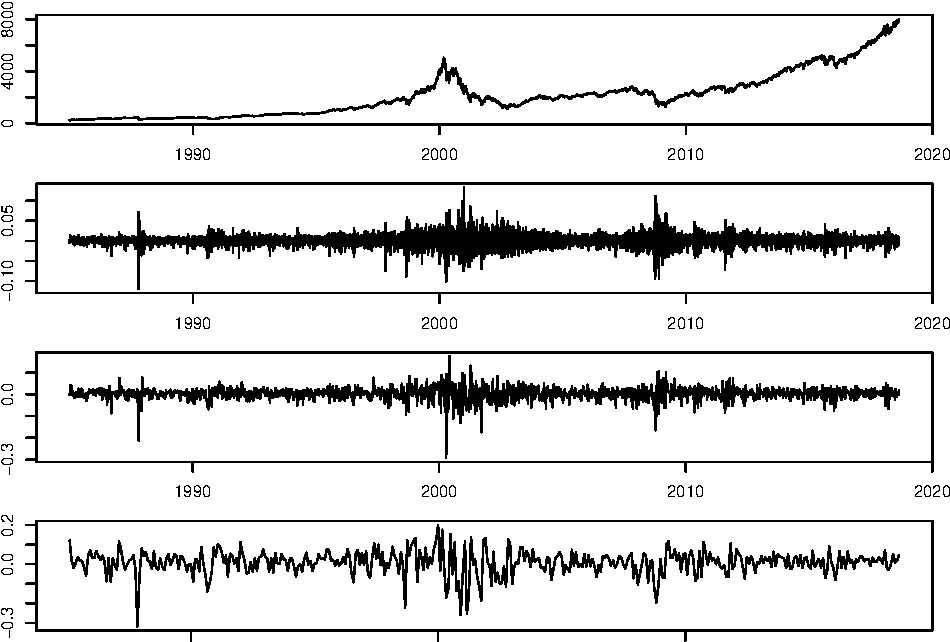
\includegraphics{hw1_files/figure-latex/unnamed-chunk-3-1.pdf}

Histograms for NASDAQ:

\begin{Shaded}
\begin{Highlighting}[]
\KeywordTok{par}\NormalTok{(}\DataTypeTok{mar=}\KeywordTok{c}\NormalTok{(}\DecValTok{2}\NormalTok{,}\DecValTok{3}\NormalTok{,}\DecValTok{2}\NormalTok{,}\DecValTok{1}\NormalTok{),}\DataTypeTok{mfrow=}\KeywordTok{c}\NormalTok{(}\DecValTok{2}\NormalTok{,}\DecValTok{3}\NormalTok{))}
\KeywordTok{hist}\NormalTok{(daily, }\DataTypeTok{probability=}\NormalTok{T, }\DataTypeTok{nclass=}\DecValTok{35}\NormalTok{, }\DataTypeTok{xlab=}\StringTok{''}\NormalTok{,}
\DataTypeTok{col=}\StringTok{"orange"}\NormalTok{,}\DataTypeTok{main=}\StringTok{"Daily returns"}\NormalTok{)}
\NormalTok{x <-}\StringTok{ }\KeywordTok{seq}\NormalTok{(}\OperatorTok{-}\FloatTok{0.5}\NormalTok{, }\FloatTok{0.2}\NormalTok{, }\FloatTok{0.01}\NormalTok{)}
\KeywordTok{lines}\NormalTok{(x, }\KeywordTok{dnorm}\NormalTok{(x, }\KeywordTok{mean}\NormalTok{(daily), }\KeywordTok{sd}\NormalTok{(daily)), }\DataTypeTok{col=}\StringTok{"blue"}\NormalTok{)}
\KeywordTok{hist}\NormalTok{(weekly, }\DataTypeTok{probability=}\NormalTok{T, }\DataTypeTok{nclass=}\DecValTok{40}\NormalTok{, }\DataTypeTok{xlab=}\StringTok{''}\NormalTok{, }\DataTypeTok{col=}\StringTok{"orange"}\NormalTok{,}
\DataTypeTok{main=}\StringTok{"Weekly returns"}\NormalTok{)}
\KeywordTok{lines}\NormalTok{(x, }\KeywordTok{dnorm}\NormalTok{(x, }\KeywordTok{mean}\NormalTok{(weekly), }\KeywordTok{sd}\NormalTok{(weekly)), }\DataTypeTok{col=}\StringTok{"blue"}\NormalTok{)}
\KeywordTok{hist}\NormalTok{(monthly, }\DataTypeTok{probability=}\NormalTok{T, }\DataTypeTok{nclass=}\DecValTok{30}\NormalTok{, }\DataTypeTok{xlab=}\StringTok{''}\NormalTok{, }\DataTypeTok{col=}\StringTok{"orange"}\NormalTok{, }\DataTypeTok{main=}\StringTok{"Monthly returns"}\NormalTok{)}
\KeywordTok{lines}\NormalTok{(x, }\KeywordTok{dnorm}\NormalTok{(x, }\KeywordTok{mean}\NormalTok{(monthly), }\KeywordTok{sd}\NormalTok{(monthly)), }\DataTypeTok{col=}\StringTok{"blue"}\NormalTok{)}
\CommentTok{# now add in qq plots}
\KeywordTok{qqnorm}\NormalTok{(daily,}\DataTypeTok{xlab=}\StringTok{'Normal quantile'}\NormalTok{, }\DataTypeTok{ylab=}\StringTok{'Quantile of daily returns'}\NormalTok{,}
\DataTypeTok{col=}\StringTok{"brown"}\NormalTok{)}
\KeywordTok{qqline}\NormalTok{(daily, }\DataTypeTok{col=}\StringTok{"blue"}\NormalTok{)}
\KeywordTok{qqnorm}\NormalTok{(weekly,}\DataTypeTok{xlab=}\StringTok{'Normal quantile'}\NormalTok{, }\DataTypeTok{ylab=}\StringTok{'Quantile of weekly returns'}\NormalTok{,}
\DataTypeTok{col=}\StringTok{"brown"}\NormalTok{)}
\KeywordTok{qqline}\NormalTok{(weekly, }\DataTypeTok{col=}\StringTok{"blue"}\NormalTok{)}
\KeywordTok{qqnorm}\NormalTok{(monthly,}\DataTypeTok{xlab=}\StringTok{'Normal quantile'}\NormalTok{, }\DataTypeTok{ylab=}\StringTok{'Quantile of monthly returns'}\NormalTok{,}
\DataTypeTok{col=}\StringTok{"brown"}\NormalTok{)}
\KeywordTok{qqline}\NormalTok{(monthly, }\DataTypeTok{col=}\StringTok{"blue"}\NormalTok{)}
\end{Highlighting}
\end{Shaded}

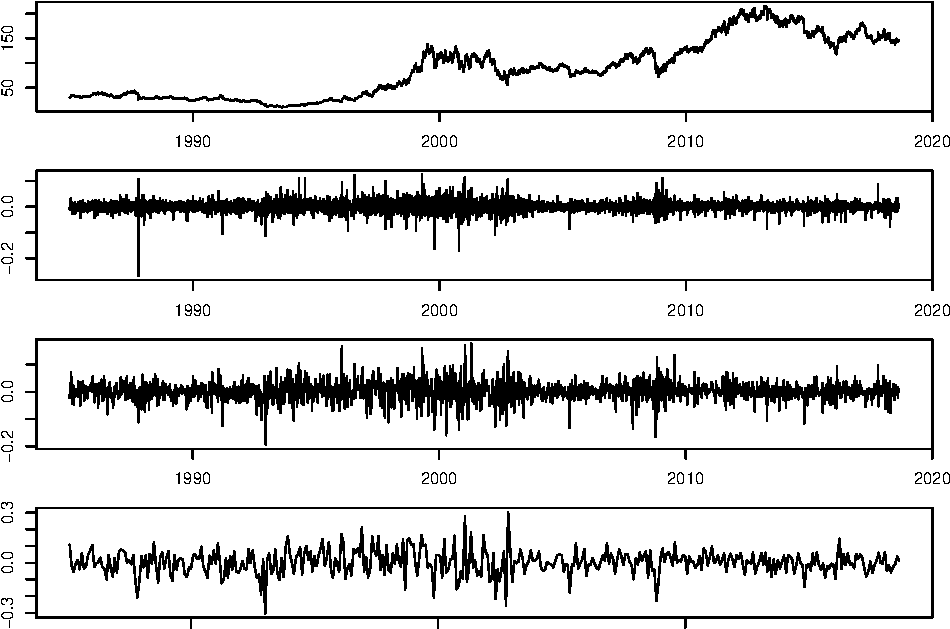
\includegraphics{hw1_files/figure-latex/unnamed-chunk-4-1.pdf}

Autocorrelations for NASDAQ:

\begin{Shaded}
\begin{Highlighting}[]
\KeywordTok{par}\NormalTok{(}\DataTypeTok{mar=}\KeywordTok{c}\NormalTok{(}\DecValTok{3}\NormalTok{,}\DecValTok{4}\NormalTok{,}\DecValTok{3}\NormalTok{,}\DecValTok{1}\NormalTok{),}\DataTypeTok{mfrow=}\KeywordTok{c}\NormalTok{(}\DecValTok{3}\NormalTok{,}\DecValTok{3}\NormalTok{), }\DataTypeTok{mgp=}\KeywordTok{c}\NormalTok{(}\FloatTok{1.8}\NormalTok{,}\FloatTok{0.5}\NormalTok{,}\DecValTok{0}\NormalTok{)) }

\KeywordTok{acf}\NormalTok{(daily,  }\DataTypeTok{main=}\StringTok{'Daily returns'}\NormalTok{)}
\KeywordTok{acf}\NormalTok{(weekly, }\DataTypeTok{main=}\StringTok{'Weekly returns'}\NormalTok{)}
\KeywordTok{acf}\NormalTok{(monthly, }\DataTypeTok{main=}\StringTok{'Monthly returns'}\NormalTok{)}
\KeywordTok{acf}\NormalTok{(daily}\OperatorTok{*}\NormalTok{daily, }\DataTypeTok{main=}\StringTok{'Squared daily returns'}\NormalTok{)}
\KeywordTok{acf}\NormalTok{(weekly}\OperatorTok{*}\NormalTok{weekly, }\DataTypeTok{main=}\StringTok{'Squared weekly returns'}\NormalTok{)}
\KeywordTok{acf}\NormalTok{(monthly}\OperatorTok{*}\NormalTok{monthly, }\DataTypeTok{main=}\StringTok{'Squared monthly returns'}\NormalTok{)}
\KeywordTok{acf}\NormalTok{(}\KeywordTok{abs}\NormalTok{(daily), }\DataTypeTok{main=}\StringTok{'Absolute daily returns'}\NormalTok{)}
\KeywordTok{acf}\NormalTok{(}\KeywordTok{abs}\NormalTok{(weekly),  }\DataTypeTok{main=}\StringTok{'Absolute weekly returns'}\NormalTok{)}
\KeywordTok{acf}\NormalTok{(}\KeywordTok{abs}\NormalTok{(monthly), }\DataTypeTok{main=}\StringTok{'Absolute monthly returns'}\NormalTok{)}
\end{Highlighting}
\end{Shaded}

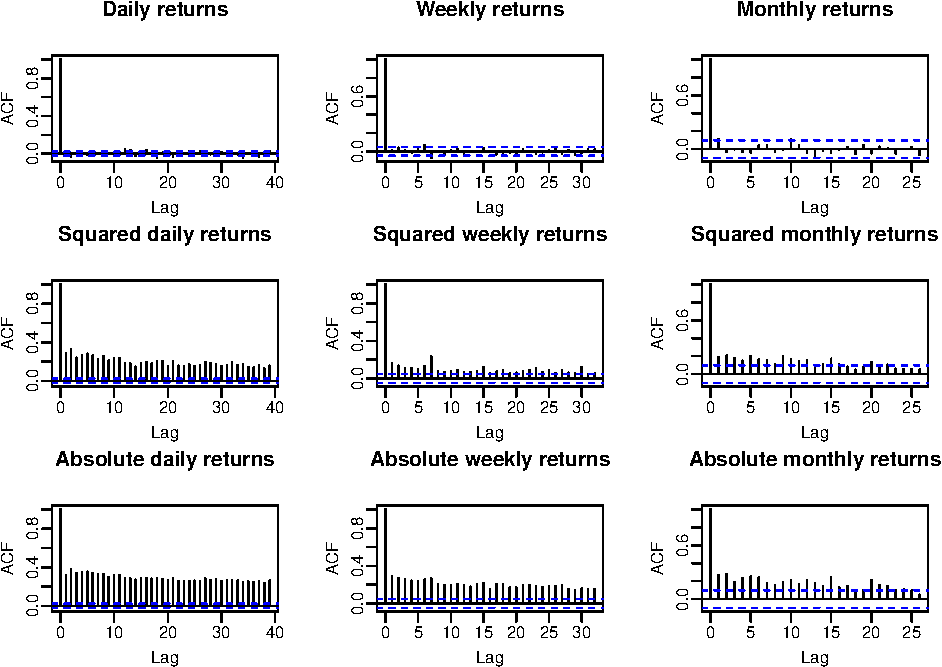
\includegraphics{hw1_files/figure-latex/unnamed-chunk-5-1.pdf}

For IBM:

\begin{Shaded}
\begin{Highlighting}[]
\CommentTok{# Extract}
\NormalTok{daily <-}\StringTok{ }\KeywordTok{log}\NormalTok{(}\KeywordTok{dailyReturn}\NormalTok{(IBM)}\OperatorTok{+}\DecValTok{1}\NormalTok{)}
\NormalTok{weekly <-}\StringTok{ }\KeywordTok{log}\NormalTok{(}\KeywordTok{weeklyReturn}\NormalTok{(IBM)}\OperatorTok{+}\DecValTok{1}\NormalTok{)}
\NormalTok{monthly <-}\StringTok{ }\KeywordTok{log}\NormalTok{(}\KeywordTok{monthlyReturn}\NormalTok{(IBM)}\OperatorTok{+}\DecValTok{1}\NormalTok{)}
\CommentTok{# Plot }
\KeywordTok{par}\NormalTok{(}\DataTypeTok{mar=}\KeywordTok{c}\NormalTok{(}\DecValTok{1}\NormalTok{,}\DecValTok{3}\NormalTok{,}\DecValTok{2}\NormalTok{,}\DecValTok{1}\NormalTok{),}\DataTypeTok{mfrow=}\KeywordTok{c}\NormalTok{(}\DecValTok{4}\NormalTok{,}\DecValTok{1}\NormalTok{)) }
\KeywordTok{plot}\NormalTok{(}\KeywordTok{index}\NormalTok{(IBM), }\KeywordTok{as.numeric}\NormalTok{(IBM}\OperatorTok{$}\NormalTok{IBM.Close), }\DataTypeTok{type =} \StringTok{"l"}\NormalTok{, }
     \DataTypeTok{ylab =} \StringTok{"daily price"}\NormalTok{)}
\KeywordTok{plot}\NormalTok{(}\KeywordTok{index}\NormalTok{(daily), daily, }\DataTypeTok{type =} \StringTok{"l"}\NormalTok{, }
     \DataTypeTok{ylab=}\StringTok{"daily log return"}\NormalTok{)}
\KeywordTok{plot}\NormalTok{(}\KeywordTok{index}\NormalTok{(weekly), weekly, }\DataTypeTok{type =} \StringTok{"l"}\NormalTok{,}
     \DataTypeTok{ylab=}\StringTok{"weekly log return"}\NormalTok{)}
\KeywordTok{plot}\NormalTok{(}\KeywordTok{index}\NormalTok{(monthly), monthly, }\DataTypeTok{type =} \StringTok{"l"}\NormalTok{, }
     \DataTypeTok{ylab=}\StringTok{"monthly log return"}\NormalTok{)}
\end{Highlighting}
\end{Shaded}

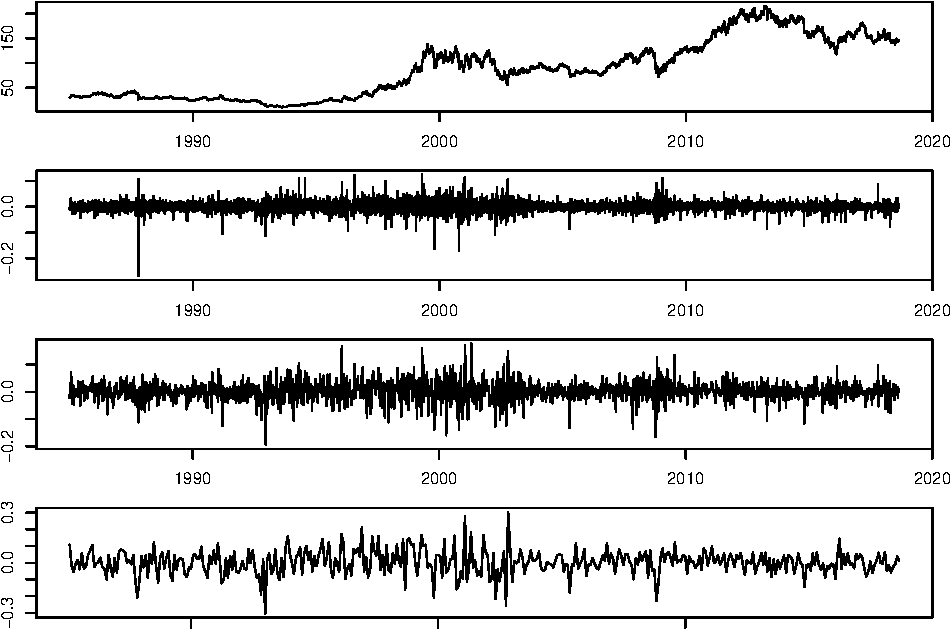
\includegraphics{hw1_files/figure-latex/unnamed-chunk-6-1.pdf}

Histograms for IBM:

\begin{Shaded}
\begin{Highlighting}[]
\KeywordTok{par}\NormalTok{(}\DataTypeTok{mar=}\KeywordTok{c}\NormalTok{(}\DecValTok{2}\NormalTok{,}\DecValTok{3}\NormalTok{,}\DecValTok{2}\NormalTok{,}\DecValTok{1}\NormalTok{),}\DataTypeTok{mfrow=}\KeywordTok{c}\NormalTok{(}\DecValTok{2}\NormalTok{,}\DecValTok{3}\NormalTok{))}
\KeywordTok{hist}\NormalTok{(daily, }\DataTypeTok{probability=}\NormalTok{T, }\DataTypeTok{nclass=}\DecValTok{35}\NormalTok{, }\DataTypeTok{xlab=}\StringTok{''}\NormalTok{,}
\DataTypeTok{col=}\StringTok{"orange"}\NormalTok{,}\DataTypeTok{main=}\StringTok{"Daily returns"}\NormalTok{)}
\NormalTok{x <-}\StringTok{ }\KeywordTok{seq}\NormalTok{(}\OperatorTok{-}\FloatTok{0.5}\NormalTok{, }\FloatTok{0.2}\NormalTok{, }\FloatTok{0.01}\NormalTok{)}
\KeywordTok{lines}\NormalTok{(x, }\KeywordTok{dnorm}\NormalTok{(x, }\KeywordTok{mean}\NormalTok{(daily), }\KeywordTok{sd}\NormalTok{(daily)), }\DataTypeTok{col=}\StringTok{"blue"}\NormalTok{)}
\KeywordTok{hist}\NormalTok{(weekly, }\DataTypeTok{probability=}\NormalTok{T, }\DataTypeTok{nclass=}\DecValTok{40}\NormalTok{, }\DataTypeTok{xlab=}\StringTok{''}\NormalTok{, }\DataTypeTok{col=}\StringTok{"orange"}\NormalTok{,}
\DataTypeTok{main=}\StringTok{"Weekly returns"}\NormalTok{)}
\KeywordTok{lines}\NormalTok{(x, }\KeywordTok{dnorm}\NormalTok{(x, }\KeywordTok{mean}\NormalTok{(weekly), }\KeywordTok{sd}\NormalTok{(weekly)), }\DataTypeTok{col=}\StringTok{"blue"}\NormalTok{)}
\KeywordTok{hist}\NormalTok{(monthly, }\DataTypeTok{probability=}\NormalTok{T, }\DataTypeTok{nclass=}\DecValTok{30}\NormalTok{, }\DataTypeTok{xlab=}\StringTok{''}\NormalTok{, }\DataTypeTok{col=}\StringTok{"orange"}\NormalTok{, }\DataTypeTok{main=}\StringTok{"Monthly returns"}\NormalTok{)}
\KeywordTok{lines}\NormalTok{(x, }\KeywordTok{dnorm}\NormalTok{(x, }\KeywordTok{mean}\NormalTok{(monthly), }\KeywordTok{sd}\NormalTok{(monthly)), }\DataTypeTok{col=}\StringTok{"blue"}\NormalTok{)}
\CommentTok{# now add in qq plots}
\KeywordTok{qqnorm}\NormalTok{(daily,}\DataTypeTok{xlab=}\StringTok{'Normal quantile'}\NormalTok{, }\DataTypeTok{ylab=}\StringTok{'Quantile of daily returns'}\NormalTok{,}
\DataTypeTok{col=}\StringTok{"brown"}\NormalTok{)}
\KeywordTok{qqline}\NormalTok{(daily, }\DataTypeTok{col=}\StringTok{"blue"}\NormalTok{)}
\KeywordTok{qqnorm}\NormalTok{(weekly,}\DataTypeTok{xlab=}\StringTok{'Normal quantile'}\NormalTok{, }\DataTypeTok{ylab=}\StringTok{'Quantile of weekly returns'}\NormalTok{,}
\DataTypeTok{col=}\StringTok{"brown"}\NormalTok{)}
\KeywordTok{qqline}\NormalTok{(weekly, }\DataTypeTok{col=}\StringTok{"blue"}\NormalTok{)}
\KeywordTok{qqnorm}\NormalTok{(monthly,}\DataTypeTok{xlab=}\StringTok{'Normal quantile'}\NormalTok{, }\DataTypeTok{ylab=}\StringTok{'Quantile of monthly returns'}\NormalTok{,}
\DataTypeTok{col=}\StringTok{"brown"}\NormalTok{)}
\KeywordTok{qqline}\NormalTok{(monthly, }\DataTypeTok{col=}\StringTok{"blue"}\NormalTok{)}
\end{Highlighting}
\end{Shaded}

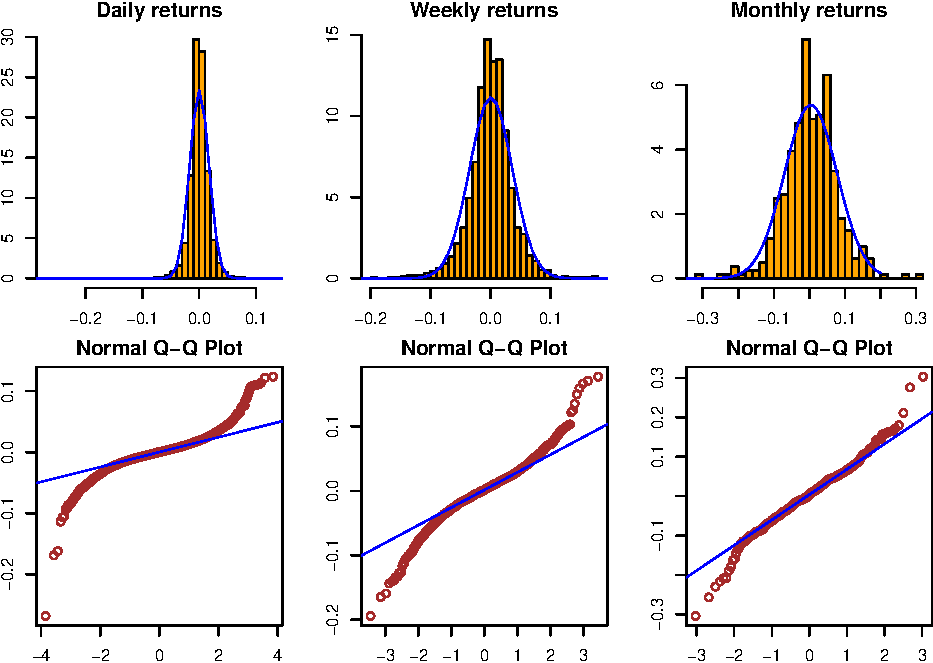
\includegraphics{hw1_files/figure-latex/unnamed-chunk-7-1.pdf}

Autocorrelations for IBM:

\begin{Shaded}
\begin{Highlighting}[]
\KeywordTok{par}\NormalTok{(}\DataTypeTok{mar=}\KeywordTok{c}\NormalTok{(}\DecValTok{3}\NormalTok{,}\DecValTok{4}\NormalTok{,}\DecValTok{3}\NormalTok{,}\DecValTok{1}\NormalTok{),}\DataTypeTok{mfrow=}\KeywordTok{c}\NormalTok{(}\DecValTok{3}\NormalTok{,}\DecValTok{3}\NormalTok{), }\DataTypeTok{mgp=}\KeywordTok{c}\NormalTok{(}\FloatTok{1.8}\NormalTok{,}\FloatTok{0.5}\NormalTok{,}\DecValTok{0}\NormalTok{)) }

\KeywordTok{acf}\NormalTok{(daily,  }\DataTypeTok{main=}\StringTok{'Daily returns'}\NormalTok{)}
\KeywordTok{acf}\NormalTok{(weekly, }\DataTypeTok{main=}\StringTok{'Weekly returns'}\NormalTok{)}
\KeywordTok{acf}\NormalTok{(monthly, }\DataTypeTok{main=}\StringTok{'Monthly returns'}\NormalTok{)}
\KeywordTok{acf}\NormalTok{(daily}\OperatorTok{*}\NormalTok{daily, }\DataTypeTok{main=}\StringTok{'Squared daily returns'}\NormalTok{)}
\KeywordTok{acf}\NormalTok{(weekly}\OperatorTok{*}\NormalTok{weekly, }\DataTypeTok{main=}\StringTok{'Squared weekly returns'}\NormalTok{)}
\KeywordTok{acf}\NormalTok{(monthly}\OperatorTok{*}\NormalTok{monthly, }\DataTypeTok{main=}\StringTok{'Squared monthly returns'}\NormalTok{)}
\KeywordTok{acf}\NormalTok{(}\KeywordTok{abs}\NormalTok{(daily), }\DataTypeTok{main=}\StringTok{'Absolute daily returns'}\NormalTok{)}
\KeywordTok{acf}\NormalTok{(}\KeywordTok{abs}\NormalTok{(weekly),  }\DataTypeTok{main=}\StringTok{'Absolute weekly returns'}\NormalTok{)}
\KeywordTok{acf}\NormalTok{(}\KeywordTok{abs}\NormalTok{(monthly), }\DataTypeTok{main=}\StringTok{'Absolute monthly returns'}\NormalTok{)}
\end{Highlighting}
\end{Shaded}

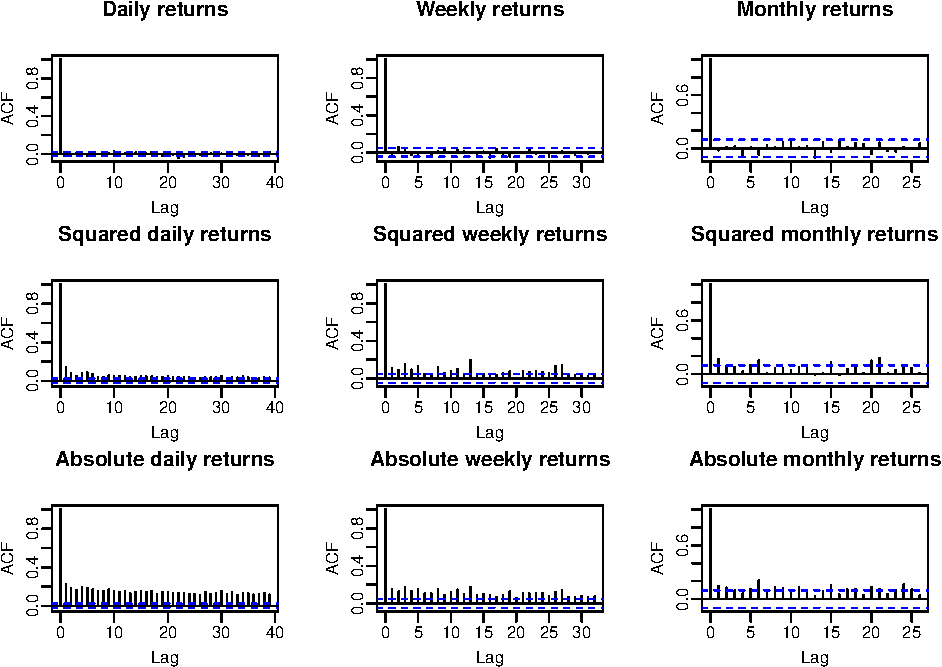
\includegraphics{hw1_files/figure-latex/unnamed-chunk-8-1.pdf}

\hypertarget{section-1}{%
\section{1.3}\label{section-1}}

Consider the following quote from Eugene Fama who was Myron Scholes'
thesis adviser: ``If the population of prices changes is strictly
normal, on the average for any stock\ldots{} an observation more than 5
standard deviations from the mean should be observed once every 7000
years. In fact such observations seem to occur about once every 3 or 5
years.'' For
\(X \sim N(\mu, \sigma^2), P(|X-\mu| > 5\sigma) = 5.733 \times 10^{-7}\),
deduce how many observations per year Fama was implicitly assuming to be
made. If a year is defined as 252 trading days and daily returns are
normal, how many years is it expected to take to get a 5 standard
deviation event? How does this answwer to the last question change when
the daily returns follow the t-distribution with 4 degrees of freedom?

\begin{Shaded}
\begin{Highlighting}[]
\KeywordTok{cat}\NormalTok{(}\StringTok{"The probability of getting this shock is 1 out of "}\NormalTok{, }
    \DecValTok{1}\OperatorTok{/}\NormalTok{(}\FloatTok{5.7333}\OperatorTok{*}\FloatTok{10e-7}\NormalTok{), }\StringTok{" days or "}\NormalTok{, }\DecValTok{1}\OperatorTok{/}\NormalTok{(}\FloatTok{5.7333}\OperatorTok{*}\FloatTok{10e-7}\NormalTok{)}\OperatorTok{/}\DecValTok{252}\NormalTok{, }\StringTok{" years"}\NormalTok{, }\StringTok{"}\CharTok{\textbackslash{}n}\StringTok{"}\NormalTok{)}
\end{Highlighting}
\end{Shaded}

\begin{verbatim}
## The probability of getting this shock is 1 out of  174419.6  days or  692.1413  years
\end{verbatim}

To get \(P(Z < -5)\):

\begin{Shaded}
\begin{Highlighting}[]
\NormalTok{p <-}\StringTok{ }\KeywordTok{pnorm}\NormalTok{(}\OperatorTok{-}\DecValTok{5}\NormalTok{) }
\KeywordTok{cat}\NormalTok{(}\StringTok{"The probability of getting this shock is 1 out of "}\NormalTok{, }
    \DecValTok{1}\OperatorTok{/}\NormalTok{p, }\StringTok{" days or "}\NormalTok{, }\DecValTok{1}\OperatorTok{/}\NormalTok{p}\OperatorTok{/}\DecValTok{252}\NormalTok{, }\StringTok{" years"}\NormalTok{, }\StringTok{"}\CharTok{\textbackslash{}n}\StringTok{"}\NormalTok{)}
\end{Highlighting}
\end{Shaded}

\begin{verbatim}
## The probability of getting this shock is 1 out of  3488556  days or  13843.48  years
\end{verbatim}

When the daily returns follow a \(t\)-distribution with 4 df:

\begin{Shaded}
\begin{Highlighting}[]
\NormalTok{p <-}\StringTok{ }\KeywordTok{pt}\NormalTok{(}\OperatorTok{-}\DecValTok{5}\NormalTok{, }\DataTypeTok{df =} \DecValTok{4}\NormalTok{) }
\KeywordTok{cat}\NormalTok{(}\StringTok{"The probability of getting this shock is 1 out of "}\NormalTok{, }
    \DecValTok{1}\OperatorTok{/}\NormalTok{p, }\StringTok{" days or "}\NormalTok{, }\DecValTok{1}\OperatorTok{/}\NormalTok{p}\OperatorTok{/}\DecValTok{252}\NormalTok{, }\StringTok{" years"}\NormalTok{, }\StringTok{"}\CharTok{\textbackslash{}n}\StringTok{"}\NormalTok{)}
\end{Highlighting}
\end{Shaded}

\begin{verbatim}
## The probability of getting this shock is 1 out of  267.0072  days or  1.059552  years
\end{verbatim}

\hypertarget{section-2}{%
\section{1.8}\label{section-2}}

According to the efficient market hypothesis, is the return of a
portfolio predictable? Is the volatility of a portfolio predictable?
State the most appropriate mathematical form of the efficient market
hypothesis.

\begin{quote}
By EMH, return of a portfolio is not predictable. The volatility is
predictable since on average it is assumed that the average change in
log price reaches the expectation \(\mu_t\). In other words, our asset
return process can be expressed as: \[
r_t = \mu_t + \epsilon_t \quad \epsilon_t \sim (0, \sigma_t^2)
\] where \(\mu_t\) is the rational expectation of the return \(r_t\) at
time \(t-1\) and \(\epsilon_t\) is the return due to unpredictable news
that arrives between \(t-1\) and \(t\). The EMH holds when: \[
E(r_t | r_{t-1}, r_{t-2}, \ldots) = E(r_t) \quad \text{almost surely}
\] In other words, \(r_t - \mu_t\) is a martingale difference with
respect the information available up to \(t-1\).
\end{quote}

\hypertarget{section-3}{%
\section{1.9}\label{section-3}}

If the Ljung-Box test is employed to test the efficient market
hypothesis, what null hypothesis is to be tested? If the autocorrelation
for the first 4 lags of the monthly log-returns of the S\&P500 is:

\[
\hat{\rho}(1) = .2, \quad \hat{\rho}(2) = -0.15, \quad \hat{\rho}(3) = 0.25, \quad \hat{\rho}(4) = 0.12
\]

based on the last 5 years of data, is the efficient market hypothesis
reasonable?

\begin{quote}
The null hypothesis tested is whether \(r_t\) is a white noise process.
The efficient market hypothesis is reasonable as shown below; we cannot
reject the white noise hypothesis for the log return data.
\end{quote}

\begin{Shaded}
\begin{Highlighting}[]
\NormalTok{Qm <-}\StringTok{ }\ControlFlowTok{function}\NormalTok{(t, rho, m)\{}
\NormalTok{  temp <-}\StringTok{ }\DecValTok{0}
  \ControlFlowTok{for}\NormalTok{(j }\ControlFlowTok{in} \DecValTok{1}\OperatorTok{:}\NormalTok{m)\{}
\NormalTok{    temp <-}\StringTok{ }\NormalTok{temp }\OperatorTok{+}\StringTok{ }\NormalTok{(}\DecValTok{1}\OperatorTok{/}\NormalTok{(t}\OperatorTok{-}\NormalTok{j))}\OperatorTok{*}\NormalTok{rho[j]}\OperatorTok{^}\DecValTok{2}
\NormalTok{  \}}
  \KeywordTok{return}\NormalTok{(}\KeywordTok{t}\NormalTok{(t}\OperatorTok{+}\DecValTok{2}\NormalTok{)}\OperatorTok{*}\NormalTok{temp)}
\NormalTok{\}}
\CommentTok{# feed in different m, find the P(Q > Qm)}
\KeywordTok{cat}\NormalTok{(}\StringTok{"When m = 1, the P( Q > Qm) is :"}\NormalTok{, }
    \DecValTok{1}\OperatorTok{-}\KeywordTok{pchisq}\NormalTok{(}\KeywordTok{Qm}\NormalTok{(}\DecValTok{60}\NormalTok{, }\KeywordTok{c}\NormalTok{(.}\DecValTok{2}\NormalTok{, }\FloatTok{-0.15}\NormalTok{, }\FloatTok{.25}\NormalTok{, }\FloatTok{.12}\NormalTok{), }\DecValTok{1}\NormalTok{), }\DataTypeTok{df =} \DecValTok{1}\NormalTok{), }\StringTok{"}\CharTok{\textbackslash{}n}\StringTok{"}\NormalTok{)}
\end{Highlighting}
\end{Shaded}

\begin{verbatim}
## When m = 1, the P( Q > Qm) is : 0.8375552
\end{verbatim}

\begin{Shaded}
\begin{Highlighting}[]
\KeywordTok{cat}\NormalTok{(}\StringTok{"When m = 2, the P( Q > Qm) is :"}\NormalTok{, }
    \DecValTok{1}\OperatorTok{-}\KeywordTok{pchisq}\NormalTok{(}\KeywordTok{Qm}\NormalTok{(}\DecValTok{60}\NormalTok{, }\KeywordTok{c}\NormalTok{(.}\DecValTok{2}\NormalTok{, }\FloatTok{-0.15}\NormalTok{, }\FloatTok{.25}\NormalTok{, }\FloatTok{.12}\NormalTok{), }\DecValTok{2}\NormalTok{), }\DataTypeTok{df =} \DecValTok{2}\NormalTok{), }\StringTok{"}\CharTok{\textbackslash{}n}\StringTok{"}\NormalTok{)}
\end{Highlighting}
\end{Shaded}

\begin{verbatim}
## When m = 2, the P( Q > Qm) is : 0.9674971
\end{verbatim}

\begin{Shaded}
\begin{Highlighting}[]
\KeywordTok{cat}\NormalTok{(}\StringTok{"When m = 3, the P( Q > Qm) is :"}\NormalTok{, }
    \DecValTok{1}\OperatorTok{-}\KeywordTok{pchisq}\NormalTok{(}\KeywordTok{Qm}\NormalTok{(}\DecValTok{60}\NormalTok{, }\KeywordTok{c}\NormalTok{(.}\DecValTok{2}\NormalTok{, }\FloatTok{-0.15}\NormalTok{, }\FloatTok{.25}\NormalTok{, }\FloatTok{.12}\NormalTok{), }\DecValTok{3}\NormalTok{), }\DataTypeTok{df =} \DecValTok{3}\NormalTok{), }\StringTok{"}\CharTok{\textbackslash{}n}\StringTok{"}\NormalTok{)}
\end{Highlighting}
\end{Shaded}

\begin{verbatim}
## When m = 3, the P( Q > Qm) is : 0.9874569
\end{verbatim}

\begin{Shaded}
\begin{Highlighting}[]
\KeywordTok{cat}\NormalTok{(}\StringTok{"When m = 4, the P( Q > Qm) is :"}\NormalTok{, }
    \DecValTok{1}\OperatorTok{-}\KeywordTok{pchisq}\NormalTok{(}\KeywordTok{Qm}\NormalTok{(}\DecValTok{60}\NormalTok{, }\KeywordTok{c}\NormalTok{(.}\DecValTok{2}\NormalTok{, }\FloatTok{-0.15}\NormalTok{, }\FloatTok{.25}\NormalTok{, }\FloatTok{.12}\NormalTok{), }\DecValTok{4}\NormalTok{), }\DataTypeTok{df =} \DecValTok{4}\NormalTok{), }\StringTok{"}\CharTok{\textbackslash{}n}\StringTok{"}\NormalTok{)}
\end{Highlighting}
\end{Shaded}

\begin{verbatim}
## When m = 4, the P( Q > Qm) is : 0.9973239
\end{verbatim}

\hypertarget{section-4}{%
\section{1.13}\label{section-4}}

Let \(S_t\) be the price of an asset at time \(t\). One version of the
EMH assumes that the prices of any asset form a martingale process in
the sense that:

\[
E(S_{t+1}|S_t, S_{t-1}, \ldots ) = S_t \quad \forall t
\]

To understand the implication of this assumption, we consider the
following simple investment strategy. With initial capital \(C_0\)
dollars, at the time \(t\) we hold \(\alpha_t\) dollars in cash and
\(\beta_t\) shares of an asset at the price \(S_t\). Hence the value of
our investment at time \(t\) is \(C_t=\alpha_t + \beta_t S_t\). Suppose
that our investment is self-financing in the sense that

\[
C_{t+1} = \alpha_t + \beta_t S_{t+1} = \alpha_{t+1} + \beta_{t+1} S_{t+1}
\]

and our investment strategy is entirely determined by the asset prices
up to the time \(t\). Show that if \(S_t\) is a martingale process,
there exist no strategies such that \(C_{t+1} > C_t\) with probability
1.

\begin{quote}
Given that
\(\alpha_t + \beta_t S_{t+1} = \alpha_{t+1} + \beta_{t+1} S_{t+1}\) must
hold and the fact that this portfolio is self-financing, we can assume
that \(C_t = \alpha_t + \beta_t S_t\). Thus, when the portfolio is
updated: \[
C_{t+1} -C_t = \beta_t (S_{t+1} - S{t})
\] and \[
E_t[C_{t+1} -C_t] = \beta_t[E(S_{t+1}) - S_t] = 0
\] Since, \(E_t(S_{t+1}) = S_t\) is a martingale process. Therefore, it
is not possible to find a strategy ensuring a strictly positive net
return with probability 1.
\end{quote}
\newpage
\singlespacing 
\end{document}
